\documentclass{article}

\usepackage{listings}
\usepackage{enumitem}
\lstset{language=bash} 
\usepackage[round]{natbib}
\usepackage{hyperref}
\usepackage{dirtree}
\usepackage{graphicx}
\graphicspath{{img/}}

\title{ARGoS-Blockchain interface}
\author{Volker Strobel \and Alex Pacheco \and Marco Dorigo}

\begin{document}
\maketitle

\begin{abstract}

  This technical report documents the installation and use of the
  ARGoS-Blockchain interface. This interface allows for conducting
  experiments in the robot swarm simulator ARGoS and the smart
  contract blockchain framework Ethereum. The blockchain part uses the
  container software Docker in order to facilitate the installation
  and the parallelization of the blockchain nodes. The use of
  blockchain-based smart contracts provides a framework for managing
  security issues in robot swarms. The interface is a convenient way
  to prototype blockchain-based control software in robot
  swarms. Byzantine robots, that is, robots that behave in an
  unintended way can disrupt the swarm behavior. In this technical
  report, we detail the motivation, setup, and usage of the
  ARGoS-blockchain interface.

\end{abstract}

\section{Introduction}

Several recent works have addressed the combination of blockchain
technology and swarm robotics
\cite{StrCasDor2018:aamas,StrDor2018:ants,StrFerDor2017:techreport-013}. This
combination proves useful for security, consensus finding, robot
economies, robot-as-a-service, and potentially many other applications
in robot swarms. However, conducting experiments involving robot
swarms and blockchain technology requires a suitable testbed. A widely
used framework consists of the Pi-puck robot platform running the
Ethereum blockchain network. However, not every researcher has access
to physical robots, obtaining and maintaining them be both
time-intense and cost-intense, not to mention the lengthy execution of
experiments. Therefore, a simulation testbed is needed to quickly try
and test different controllers and scenarios. The ARGoS robot
simulator \citep{PinTriOGr-etal2012:si} is the state-of-the-art
research platform to conduct simulations in swarm robotics. Such a
framework proves useful both for researchers who do not have access to
a suitable robot platform, such as the Pi-puck robot. Additionally, a
suitable platform is important before running time- and cost-consuming
experiments with real robots.

In general, in swarm robotics research, each robot is a blockchain
node, and contributes to the maintenance of the system by exchanges
blockchain information. To link ARGoS and blockchain software, we
developed the ARGoS-Blockchain interface that provides access to the
blockchain nodes for the robots (Figure~\ref{fig:interface}). The
interface is intended to facilitate research in blockchain-based robot
swarms by allowing to call blockchain functions in
ARGoS. Additionally, using Docker makes it easy to install and run the
interface on different platforms.


\section{Software availability}

The open-source software is available at GitHub: the blockchain module
is available at
\footnote{\url{https://github.com/Pold87/ARGoS-Blockchain-interface}}
and the ARGoS module is available at
\footnote{\url{https://github.com/Pold87/robot-swarms-need-blockchain}}.

\begin{figure}[t]%\centering
\dirtree{%
.1 geth/.
.1 img/.
.1 local\_scripts/.
.1 .gitignore.
.1 README.
.1 docker-compose.yml.
}
\label{fig:folderstructure}  
\caption{The folder structure of the package.}
\end{figure}
\begin{figure}
  \centering
    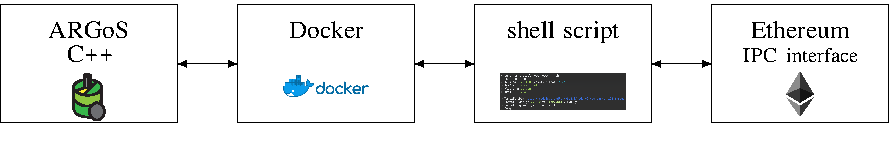
\includegraphics[width=\textwidth]{overview}
  \caption{For each robot, the ARGoS-Blockchain interface establishes
    a connection to the Ethereum blockchain via a Docker container and
    shell scripts that provide templates for executing Ethereum (geth)
    functions.}
  \label{fig:overview}  
\end{figure}

\section{Overview}

The implementation of the custom Ethereum network is based on
Capgemini \textsc{aie}'s Ethereum
Docker\footnote{\url{https://github.com/Capgemini-AIE/ethereum-docker},
  accessed on November 6, 2019}. Docker containers
\citep{Mer2014:linux} contain all the necessary dependencies to run
specific applications and are more lightweight than a virtual
machine. In our setup, for each robot, the Ethereum implementation
\emph{geth} is executed in a separate Docker container. The simulated
robots maintain a \emph{custom} Ethereum network, i.e., a network that
is shared among the simulated robots and independent of Ethereum's
main network. Different containers can communicate with each other via
channels.

In order to execute an Ethereum function (e.g., create a new smart
contract) from ARGoS, a robot uses its C\texttt{++} controller to
attach to the Docker container. The Docker containers provide shell
scripts\footnote{The interface uses shell scripts, since, during
  development, it became evident that they are executed much faster
  than other Ethereum APIs.} with customizable templates (e.g., one of
the templates compiles the smart contract, uses the binary code to
send a blockchain transactions, and waits until the contract is
mined). Via Ethereum's \textsc{ipc} (interprocess communications)
interface, the shell scripts execute the Ethereum functions.

We use an auxiliary `bootstrap' node for publishing the smart contract
to the blockchain at the beginning of each run of the simulations
(Figure~\ref{fig:initialization}). The bootstrap node then mines the
smart contract and sends the contract address and the \textsc{abi}
(application binary interface; the \textsc{abi} specifies which
functions a smart contract provides and how to call them) to the
controllers of the robots. As soon as this is done, the bootstrap node
is removed from the network. The bootstrap node is not necessarily
required and the smart contract could also be created by a
robot. However, we used an auxiliary node to make sure (i) that the
smart contract is available at the start of the actual experimental
run and (ii) that robots have the same initial conditions in all
experiments.

The experiments were conducted on a computer cluster. To simulate the
limited hardware of real robots, one core with 2.0~GHz and 1.8~GB of
memory was assigned to each Docker container\footnote{This is a
  reasonable choice as a robot's computer could easily have such
  characteristics. It is also a convenient choice because on a
  computer with 2.0~GHz and 1.8~GB of RAM, Ethereum works
  ``out-of-the-box,'' without any modifications; therefore, any
  interested user can obtain the most recent release of Ethereum from
  the official depository and use it with our publicly available
  ARGoS-Blockchain interface.}. The communication channels between the
Docker containers were only established when robots were within a
50~cm communication range in order to simulate the local communication
capabilities of real robots.

The description in this report is intended to allow everyone to run
blockchain-based robot experiments in simulation. There is no need for
specific hardware but powerful CPU and RAM are advantageous for fluent
experiments.

The ARGoS-Blockchain interface is composed of two modules. 

\subsubsection{Module~1: Blockchain part}
Module~1 allows for creating an Ethereum network with several nodes,
where each node is located in a separate Docker container. For the
ARGoS-Blockchain interface, the interaction with the Ethereum nodes is
done via C\texttt{++}, using the code in the following repository:\\
\url{https://github.com/Pold87/robot-swarms-need-blockchain}

This repository contains one module of the ARGoS-Blockchain interface
that is described in the article ``Blockchain Technology Secures Robot
Swarms: A Comparison of Consensus Protocols and Their Resilience to
Byzantine Robots by Strobel, V., Castello Ferrer, E., and Dorigo, M.''

For debugging purposes or for creating your own private Ethereum
network, you can also use this module without ARGoS.

\begin{figure}[t]
  \centering
  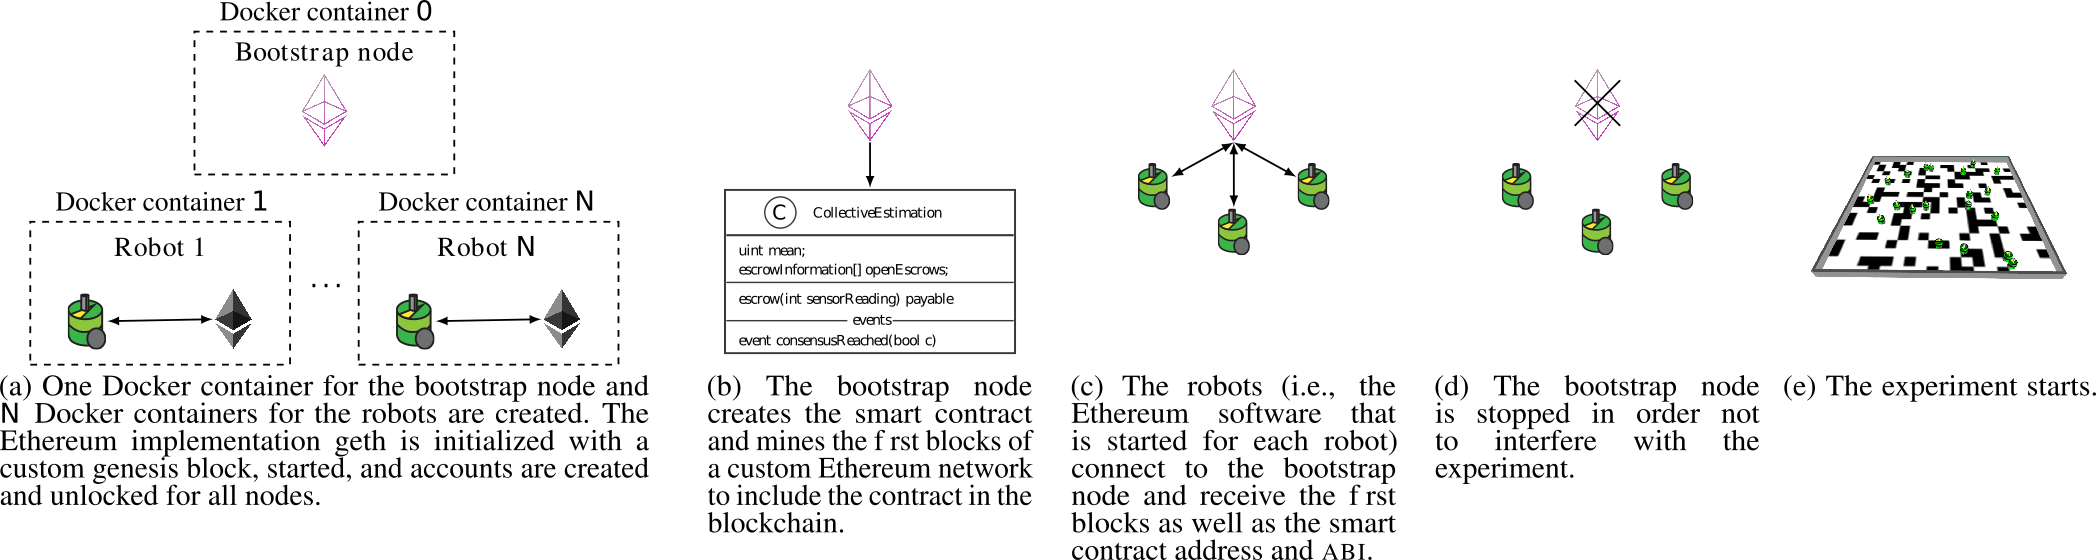
\includegraphics[width=\textwidth]{interface}
  \caption[Overview of the ARGoS-Blockchain interface]{This scheme
    gives an overview of the workflow of the ARGoS-Blockchain
    interface}
  \label{fig:interface}
\end{figure}

\subsubsection{Module~2: ARGoS part}

\section{Setup}

The following setup steps describe the installation using Linux as
operating system.

\subsection{Requirements}
\begin{itemize}
\item Sufficient disk space (at least 16 GB)
\item Docker 
\item ARGoS\footnote{\url{https://github.com/ilpincy/argos3}} and the
  ARGoS e-puck robot
  plugin\footnote{\url{https://github.com/demiurge-project/argos3-epuck}}
  (carefully read the instructions on the respective respositories)
\end{itemize}

\subsection{Obtain Source Code}

\begin{enumerate}[leftmargin=*]
\item Create a base folder for storing the two modules of the
  ARGoS-Blockchain interface.
\begin{verbatim}
$ mkdir interface/
$ cd interface/
$ pwd
/home/vstrobel/software/interface
\end{verbatim}

\item Obtain the source code for the blockchain module.
\begin{verbatim}
$ git clone https://github.com/Pold87/ARGoS-Blockchain-interface
\end{verbatim}

\item Obtain the source code for the ARGoS module.
\begin{verbatim}
git clone https://github.com/Pold87/robot-swarms-need-blockchain"
\end{verbatim}
\end{enumerate}

\subsection{Installation --- Module~1: Blockchain module}

\begin{enumerate}[leftmargin=*]
\item By default, the execution of Docker commands requires root user
  privileges. To facilitate the execution of Docker commands, it is
  possible to run Docker as non-root user (i.e., without
  \texttt{sudo}) as follows (see
  \url{https://docs.docker.com/engine/install/linux-postinstall/} for
  more detailed instructions).
\begin{verbatim}
$ sudo groupadd docker
$ sudo usermod -aG docker $USER
\end{verbatim}
 % New item
\item Obtain the Ethereum source code and store it in the folder
\verb|myowngeth/|. Please note that Ethereum is compiled locally
here. While there are Docker images for Ethereum, this allows for more
customization (e.g., if you want to change the size of the DAG file,
as explained in Section~\ref{sec:limited-hardware}).

\begin{verbatim}
$ cd ARGoS-Blockchain-interface/ && cd geth/
$ git clone https://github.com/ethereum/go-ethereum.git myowngeth/
\end{verbatim}
% New item
\item Create the Ethereum image and initialize the Docker swarm.

\begin{verbatim}
$ docker build -t mygeth .
$ docker swarm init
\end{verbatim}
% New item
\item Set the ARGoS folder in the file \verb|start_network.sh|.

\begin{verbatim}
$ nano ../local_scripts/start_network
ARGOSFOLDER="/home/vstrobel/software/interface/robot-swarms-need-blockchain"
\end{verbatim}
% TODO: Run script with NUMROBOTS=0
\end{enumerate}
\subsection{Installation --- Module~2: ARGoS module}

\item Compile the ARGoS code.
\begin{verbatim}
$ cd /home/vstrobel/software/interface/robot-swarms-need-blockchain/
$ mkdir build/
$ cd build/
$ cmake ..
$ make
\end{verbatim}
  
\item Set the variable \verb|DOCKERBASE| in the file
\verb|global_config.sh| to the full path where the Blockchain module
(Module 1) repository is located on your computer, for example:

\begin{verbatim}
$ cd ..
$ nano global_config.sh
DOCKERBASE='/home/vstrobel/Documents/docker-geth-network/'
\end{verbatim}

\item In order to be able to mine, you need to create the DAG datasets as
follows (the creates files require approximately 2~GB disk space and
the execution of the script can take take several minutes):

\begin{verbatim}
cd local_scripts/
bash create_dag.sh
\end{verbatim}  
\end{enumerate}

\section{Modifications}

\subsection{Changes for limited hardware}
\label{sec:limited-hardware}

The target platform of the ARGoS-blockchain interface are robots with
limited hardware. The mining algorithm Proof-of-Work requires a 1~GB
dataset by default that must be stored in the memory. On a Pi-puck,
Proof-of-Work does not run out-of-the-box due the large DAG file that
has to be kept in memory. In order to reduce the DAG file size
(warning: this will likely decrease the security of the network in a
real-world deployment but is fine in a private testnet), modify the
file \verb|go-ethereum/consensus/ethash/algorithm.go| as described below.

1. Change
\begin{verbatim}
datasetInitBytes   = 1 << 30 // Bytes in dataset at genesis
\end{verbatim}
to
\begin{verbatim}
datasetInitBytes   = 1 << 20 // Bytes in dataset at genesis
\end{verbatim}
2. Comment out the following lines:
\begin{verbatim}
//if epoch < maxEpoch {
	  //return cacheSizes[epoch]
	  //}
\end{verbatim}
        and        
\begin{verbatim}
//if epoch < maxEpoch {
	  //return datasetSizes[epoch]
	  //}
\end{verbatim}

\section{Run}

Usually, the network is created when a swarm robotics experiment is
started, using one of the start scripts in
\url{https://github.com/Pold87/robot-swarms-need-blockchain}.

However, you can also start the Ethereum network without ARGoS, using
the following command:

\begin{verbatim}
bash local_scripts/start_network.sh <number of nodes>
\end{verbatim}

That is, \verb|bash local_scripts/start_network.sh 5|, would create a
private Ethereum network with 5 nodes.

\section{Debugging}

First, check that the Docker container for the bootstrap node and the
individual containers for the robots are running:

\begin{verbatim}

\end{verbatim}

% Mention --no-trunc and how to access logs

\section{Usage}

The functions of the interface can be found in the file
\verb|/interface/generic_interface.cpp|.


\begin{itemize}
\item \texttt{unlockAccount}: Unlock the coinbase account.
\item \texttt{startMining}: Start the mining process using one thread.
\item \texttt{stopMining}: Stop the mining process.
\item \texttt{addPeer}: Add a peer based on its enode.
\item \texttt{removePeer}: Add a peer based on its enode.
\item \texttt{scInterface}: 
\end{itemize}

\subsubsection*{Acknowledgements}

Volker Strobel and Marco Dorigo acknowledge support from the Belgian
F.R.S.-FNRS, of which they are a Research Fellow and a Research
Director respectively. Alexandre Pacheco acknowledges support from the
Faculty of Applied Sciences of the Universit\'{e} Libre de Bruxelles.


\bibliographystyle{abbrvnat}
\bibliography{library}


\end{document}
